\section{{\bf \retro} Overview}
\label{sec:ov}


\begin{figure}[t]
   \centering
   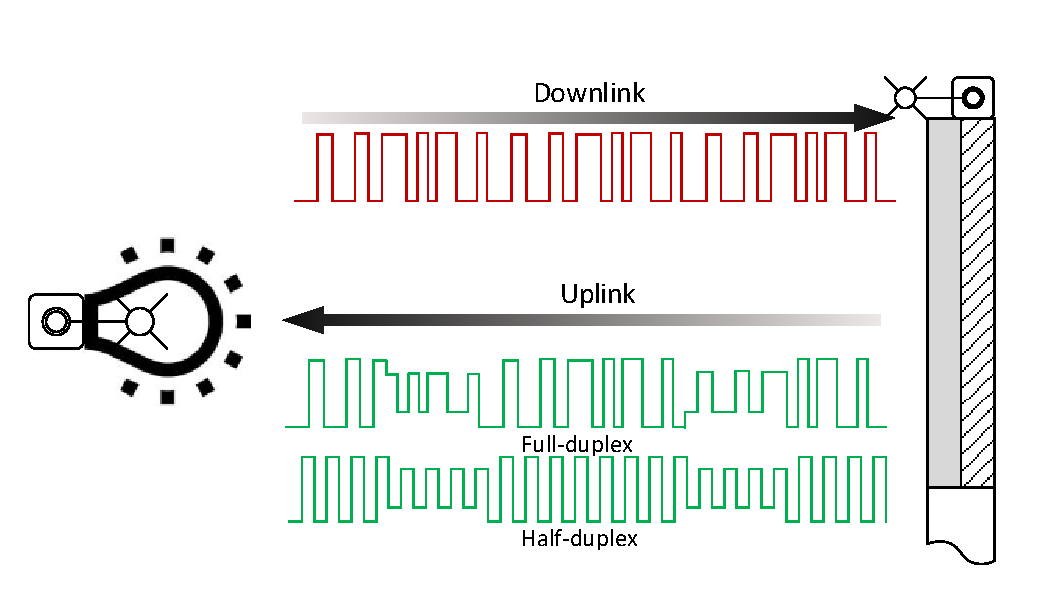
\includegraphics[width=0.9\columnwidth]{fig/link.pdf} 
   \vskip -1ex
   \caption{Concept illustration of the \retro system.}
   \label{fig:link}
   \vskip -1em
\end{figure}


The basic design of \retro\ is to backscatter the incoming light using a retro-reflector fabric and to modulate it with an LCD. The overall concept is illustrated \figref{fig:link}. which depicts how our design support both half-duplex and full-duplex modes. %The symbol length is relatively much longer than the carrier waveform. This is due to the low refreshing rate of the commercially off-the-shelf LCDs. We want to point it out upfront that, doomed by the limited refreshing rate of LCD, our design is intrinsically asymmetric with a slow uplink.  


\subsection{Challenges}
While retro-reflecting and modulating the retro-reflected light makes it possible to establish a visible light uplink from a mobile device to the illuminating infrastructure, the actual design of \retro still faces two major challenges, rooted from the practicality and the low-power requirement of the system. 

\paragraph{Weak, Noisy Reflected Signal} 
The signal collected by the light sensor collocating at the light source is weak,  about $4$ orders of magnitude weaker than the LED emission (measured with the tag at a 1.5-meter distance and a 12W LED lamp), due to the small size of the retro-reflector and relatively large working range. 
We use a photodiode with wide field of view (FoV) on the \reader to avoid constraining the range of possible tag deployment. The wide FoV of the photodiode not only makes it less sensitive to the reflected lights (as only a tiny portion of its view actually corresponds to the retro-reflecting area of a tag), but also invites severe interference from the leakage and ambient reflection of the strong downlink signal and carrier. The converted electrical signal is further interfered by the harmonics of 50Hz (or 60Hz) AC current. 

\paragraph{Energy Efficiency} 
Secondly, the low power consumption requirement of \vitag (in hope to achieve battery-free operation by only harvesting energy from the illuminating LED) entails careful design as well. 
The receiving (demodulation and decoding) unit and modulation unit (the LCD) on the \vitag consume significant energy. The LCD shutter leverages the electric field to control the arrangement of liquid crystal molecules (to polarize the light). It itself is a capacitor. 
Frequent charging and discharging the LCD consumes relatively significant energy.
Its power consumption increases linearly with the refreshing rate. In our measurement, it consumes $84\mu A$ current at a 500Hz refreshing rate.

In addition, for sake of cost and energy consumption, we do not use any high precision oscillator on the \vitag. There is no clock synchronization between a \reader and \vitag(s) either. These consideration introduces additional challenges. 



%%There is also a derived challenge caused by our desire to further push down the energy consumption of the device. As will be elaborated in Section~\ref{sec:tagtx}, we avoided using energy expensive crystal oscillator but used a simple RC oscillator to serve as the clock. The clock generated by the RC oscillator can drift in a range of \fyi{$\pm 80\%$ from the targeted frequency}. This incurs new challenge in the decoding of the uplink signal. 


\subsection{Principles}
Inspired by design principles of some recent backscattering systems \cite{abc1,abc2, abc3}, we we apply the following design principles in addressing the challenges:
\begin{Itemize}
\item Use analog components for signal detection. This is to avoid the expensive ADC and relieve the MCU from heavy digital signal processing. 
\item Make the transistors in the circuit work at a low DC operation point (\eg close to cut-off state). This is an exploitation of the nonlinear relationship between the amplification gain and DC work current (hence energy consumption) of a triode. 
%In our amplifier design, we achieve high gain by cascading multiple low-gain amplifiers in which the triode works at almost cut-off state, instead of a single amplifier with large working current. 
%\todo{Need verification on the correctness! Need to draw the working curve of a triode?}
\item Reuse energy as much as possible. This is particularly to reduce LCD energy consumption.
\end{Itemize}


\iffalse
\begin{figure*}[t]
  \begin{center}
        \includegraphics[width=\textwidth]{../illustrations/ReadAndTag.eps}
      \vspace{-2em}
      \caption{\retro system diagram. The left part is the \reader and the right part is the \vitag. }\label{fig:sysdiagram}
  \end{center}
\end{figure*}
\else
\begin{figure}[t]
  \begin{center}
        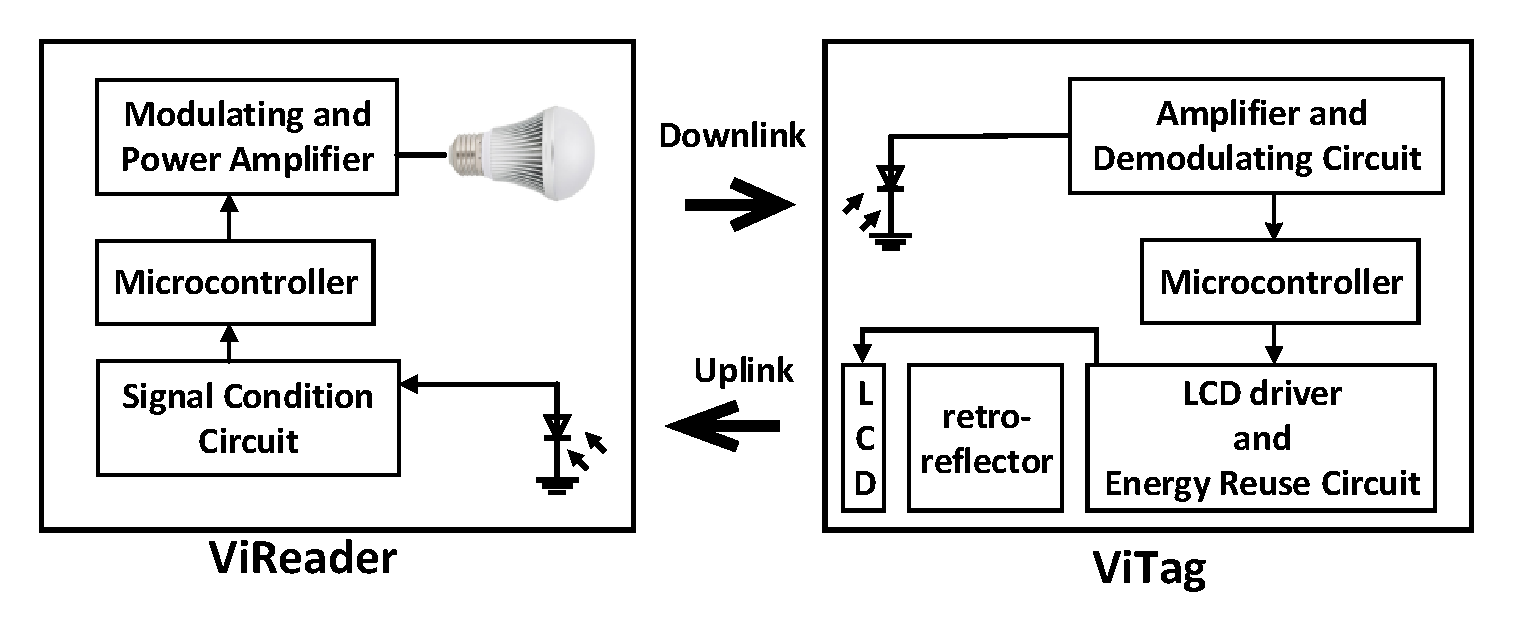
\includegraphics[width=\columnwidth]{fig/reader_tag_simplified.pdf}
      \vspace{-2em}
      \caption{\retro system block diagram.}\label{fig:sysdiagram}
  \end{center}
\end{figure}
\fi


\subsection{Design Overview}
\figref{fig:sysdiagram} shows the architecture of a \retro system. It consists of a \reader and a \vitag. The \reader resides on the lighting infrastructure, consisting of an illumination LED and transmission logic (termed \readertx hereafter), a light sensor and the subsequent receiving circuit (\readerrx). The \vitag\ consists of a light sensor and receiving circuits (\tagrx), and a retro-reflector, a modulating LCD and other circuitry components (\tagtx).  The \readertx and \tagrx together make the \textit{downlink} visible light channel, and the \tagtx and \readerrx together make the \textit{uplink}. 
\retro operates as follows: 

\paragraph{Downlink} 
For the downlink communication, the \reader sends out information by modulating the carrier using On/Off Keying (OOK) and employing Manchester coding. This signal is captured by the light sensor of \vitag, amplified, demodulated and decoded by \tagrx in analog domain.

\paragraph{Uplink} 
As for the uplink communication, the MCU on the \vitag controls the LCD to modulate the light carrier reflected by the retro-reflector fabric. The reflected light travels back to the light sensor that collocates with the LED. Upon capture, the weak signal is first amplified with a differential amplifier to mitigate noises, further amplified, demodulated, digitized and finally decoded. Special logic has been designed to account for the possible clock drift at the \vitag when modulating the reflected carrier as we have used a cheap RC oscillator to avoid high energy cost and overly large size of crystal oscillators. 

The downlink and uplink can work concurrently on their respective bands. Hence it is capable of full-duplexing. 
Normally, when there is no traffic, the \readertx sends out the carrier by switching the LED light at a high frequency $f_0$, which should be fast enough to avoid perceivable flickering (i.e., $f_0 \gg 200$Hz). In our implementation, we set $f_0$ to $1MHz$. We support dimming of the LED by changing its DC bias. Both the receiving logic on \reader and \vitag (when turned on) keep on monitoring their own incoming light channel. With this design, a \vitag can initiate the communication to the \reader. An alternative design would be turning on the \tagtx only when \vitag\ receives certain information. This is the half-duplexing mode where only the \reader can initiate a communication session, similar to how existing RFID system works.


%In the text below, we describe our design of the \retro system in more detail. As the \readertx is of a standard design -- using an MCU to perform encoding and control the power amplifier to toggle on/off of the LED light. The concrete design choices are that we employ a 1MHz carrier,\footnote{This is a limitation from commercial off-the-shelf LED we have. If we toggle at a faster rate, the amplitude difference between On and Off state will be too small to serve as an effective carrier.} use Manchester coding and perform OOK.  We thus focus on the design of the other three components, namely \readerrx, \tagtx, and \tagrx., elaborating the key design choices.  \q{In one of the versions, we mentioned the bandwith of 100kHz. What does this number matter?}

